\chapter{System Design}
This chapter delineates the overall architecture of the simulation platform, the selection of key technologies, and the rationale behind these design choices. A well-designed and scientifically sound simulation platform is the cornerstone for ensuring the validity and credibility of the research findings.

The primary objective of this system design is to create a testbed that can reliably replicate the workflow of the Johnson Draft and flexibly simulate various space network environments. To this end, the design adheres to the following core principles:

\begin{itemize}
    \item Modularity: The system is partitioned into functionally independent subsystems (e.g., servers, users) to facilitate the configuration and testing of different use cases.
    \item Reproducibility: Containerization technology is employed to ensure that the entire experimental environment can be precisely and consistently reconstructed, guaranteeing the scientific validity of the results.
    \item Authenticity: The platform utilizes industry-standard, real-world software (e.g., Postfix, Thunderbird) rather than simplified scripts to simulate application scenarios as authentically as possible.
    \item Controllability: The network environment, particularly parameters like delay and disruption, must be quantifiable and precisely controllable to provide a solid basis for performance analysis.
\end{itemize}

\section{System Architecture}

To achieve the aforementioned objectives, this dissertation employs a five-node simulation model built on Docker containers. The overall architecture, which simulates two logically separate network regions—the ``Earth Internet'' and the ``Moon Internet''—is depicted in Figure~\ref{fig:system-architecture}. These two regions are interconnected by a simulated DTN link characterized by long latency.

\begin{figure}[h]
    \centering
    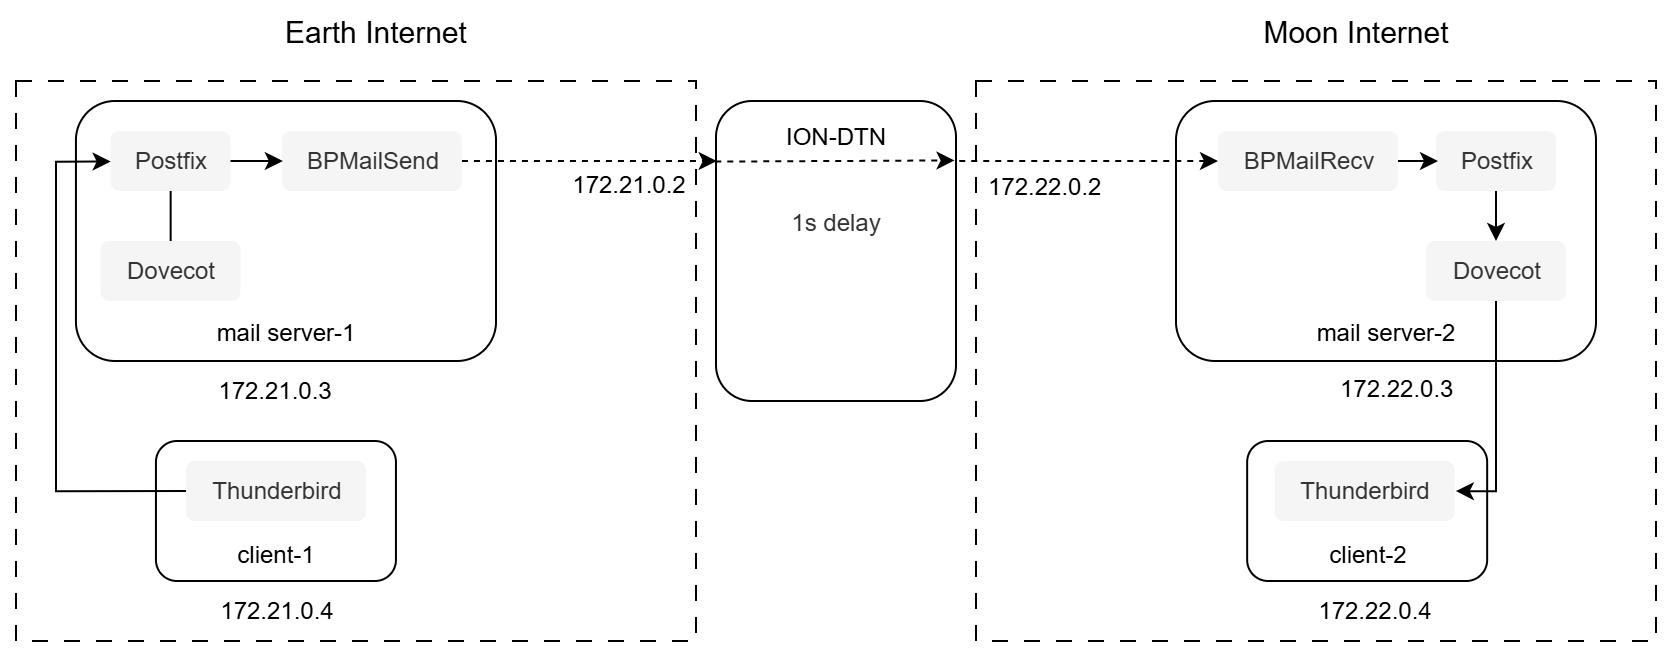
\includegraphics[width=1.0\textwidth]{Experimental Methods/Simulation_Johnson.png}
    \caption{System Architecture Diagram}
    \label{fig:system-architecture}
\end{figure}

\subsection*{Logical Zones}
\begin{itemize}
    \item Earth Internet
    
    This zone comprises the \texttt{mail-server-1} (IP: 172.21.0.3) and \texttt{client-1} (IP: 172.21.0.4) containers, both residing on the 172.21.0.0/24 subnet. They simulate the mail server and user terminal on Earth.
    \item Moon Internet
    
    This zone includes the \texttt{mail-server-2} (IP: 172.22.0.3) and \texttt{client-2} (IP: 172.22.0.4) containers on the 172.22.0.0/24 subnet, simulating the corresponding facilities on the Moon.
\end{itemize}

\subsection*{Core Component Roles}
\begin{itemize}
    \item Mail Servers (\texttt{mail-server-1}, \texttt{mail-server-2}): Act as the core of their respective network zones, responsible for email transmission, reception, and storage. They are deployed with a complete mail service suite and the DTN gateway functionality.
    \item User Terminals (\texttt{client-1}, \texttt{client-2}): Simulate end-users interacting with their respective local mail servers via standard email client software.
    \item Delay Node: Acts as a network impairment simulator, bridging the Earth and Moon networks. All inter-regional traffic must traverse this node, enabling application of controlled delays and disruptions.
\end{itemize}

\subsection*{Data Flow Example (Earth to Moon)}
\begin{enumerate}
    \item The user on \texttt{client-1} composes an email in Thunderbird and sends it via SMTP to Postfix on \texttt{mail-server-1}.
    \item Postfix hands the email to the local BPMailSend component.
    \item BPMailSend encapsulates the email into a DTN bundle and sends it to the Delay Node.
    \item After the configured delay, the Delay Node forwards the bundle to \texttt{mail-server-2}.
    \item BPMailRecv on \texttt{mail-server-2} decapsulates the bundle and restores the original email.
    \item The email is delivered to Postfix, stored by Dovecot, and retrieved by \texttt{client-2} via IMAP.
\end{enumerate}

This partitioned architecture clearly simulates a multi-node, cross-network distributed communication scenario, providing a solid foundation for subsequent simulation analysis.

\section{Simulation Environment and Technology Selection}

\subsection{Docker}
Docker was selected as the underlying platform for this simulation experiment. As an open-source application container engine, Docker allows packaging applications and dependencies into a portable container. This choice offers advantages in isolation, reproducibility, and resource efficiency.

\subsubsection*{Lightweight Virtualization and Resource Efficiency}
Unlike traditional virtual machines, Docker containers share the host OS kernel, avoiding the overhead of a full OS per instance. This enables near-instant startup times and supports running multiple nodes concurrently on one physical host~\cite{Docker}.

\subsubsection*{Environmental Isolation and Consistency}
Docker provides isolated filesystems, processes, and networking for each container, preventing conflicts such as port clashes or dependency issues—particularly useful when running multiple instances of Postfix or ION.

\subsubsection*{Guaranteed Scientific Reproducibility}
Through Dockerfiles and Docker Compose, the environment is defined as code, ensuring identical experimental setups across different machines~\cite{DockerRepo}.

\subsection{Comparison with Other Schemes} \label{sec:comparison}
The selection of an appropriate methodology for the simulation platform is a critical step in the system design phase, as it directly influences the reproducibility, scalability, and experimental control of the research. In developing the testbed for this dissertation, three primary approaches were considered: traditional virtualization using virtual machines, a physical hardware deployment, and OS-level virtualization, or containerization. This section provides a comparative analysis of these approaches to justify the selection of Docker as the foundational technology.

\subsubsection*{Comparison with a Linux Virtual Machine (VM) Scheme}
\begin{itemize}
    \item Resource Overhead
    
    A significant drawback of a VM-based approach is the substantial resource overhead. Running five independent Linux VMs would require immense memory and disk allocation, as each VM encapsulates a complete guest operating system. In contrast, Docker containers share the host machine's OS kernel, making them exceptionally lightweight~\cite{DockerPerfComp}. This lower resource footprint makes it feasible to conduct complex, multi-node experiments on a standard personal computer or a single server.
    \item Deployment Efficiency
    
    The efficiency of deployment and iteration is another key differentiator. Creating and configuring a VM is a time-consuming process, often taking several minutes or longer. Conversely, a Docker container can be launched from a cached image in a matter of seconds. This rapid deployment cycle is particularly advantageous during the iterative development and debugging phases of research, where environments must be frequently rebuilt and adjusted.
\end{itemize}

\subsubsection*{Comparison with a Physical Hardware (Raspberry Pi) Scheme}
The use of physical hardware, such as multiple Raspberry Pi devices, was employed by researchers in the ``SMTP Gatewaying Across Delay Tolerant Networks'' project. While this method offers a tangible and intuitive representation of a physical network, a Docker-based approach was deemed more suitable for the objectives of this dissertation.

\begin{itemize}
    \item Cost and Scalability
    
    A physical hardware setup involves logistical overhead, including the procurement, deployment, and maintenance of multiple devices and their corresponding network accessories. This approach incurs higher costs and is not easily scalable. The Docker solution, however, allows for the simulation of a virtually unlimited number of nodes on a single host machine at minimal cost, offering superior scalability.
    \item Control and Consistency
    
    Physical hardware is susceptible to confounding variables, such as inconsistent network cable quality, power supply fluctuations, and SD card performance. Docker, on the other hand, provides a purely software-defined and highly controlled virtual environment. It allows for the precise management of network topology and parameters, effectively eliminating physical-world variables and making it the superior choice for scientific simulations that require rigorous control over experimental conditions.
\end{itemize}

In conclusion, while both VMs and physical hardware are viable for certain types of network experimentation, the containerization approach with Docker offered the optimal balance of resource efficiency, deployment speed, scalability, and experimental control. Its ability to provide a consistent, reproducible, and precisely controlled software-defined environment made it the most suitable methodology for this dissertation.

\section{Email System Design}

\begin{itemize}
    \item Postfix (MTA)
    
    Chosen for security, stability, and performance. Provides a flexible interface for integrating BPMail via configuration files.
    \item Dovecot (MDA/IMAP Server)
    
    High-performance, secure, and integrates seamlessly with Postfix.
    \item Thunderbird (MUA)
    
    Real-world client generating realistic emails, improving simulation authenticity.
\end{itemize}

\section{Delay-Tolerant Networking Design}
\subsection{Interplanetary Overlay Network (ION)}
The ION is an open-source software suite developed by NASA's Jet Propulsion Laboratory (JPL) to implement the DTN architecture. With significant space-flight heritage from numerous deep-space and near-Earth missions, ION is designed for robust operation in challenged communication environments characterized by long delays and frequent link disruptions~\cite{burleigh2007interplanetary}. Architecturally, ION provides a mature implementation of the Bundle Protocol. Key services within the ION suite include a variety of Convergence Layer Adapters (e.g., TCPCL, UDPCL, LTP) to operate over different underlying links, and security extensions via the Bundle Protocol Security (BPSec) specification.

\subsection{Comparison with Other DTN Protocol Stack}
For this dissertation, ION was selected as the DTN implementation after a comparative evaluation against other alternatives. The selection is justified by three primary factors: technical completeness, academic precedent, and practical feasibility.

\subsubsection*{Technical Completeness}
In terms of technical completeness, ION offers the features required by this dissertation. A comparative analysis of leading DTN stacks (Table \ref{tab:DTN_Stacks}), adapted from and extended by Ronny L. Bull et al.~\cite{bull2024network} based on the Internet Society Interplanetary Chapter~\cite{ipnsig2023_home} Pilot Projects Working Group’s analysis~\cite{ipnsig2023_bp_impl}, highlights ION's extensive support for the BP core specifications.

\begin{table}[htbp]
\centering
\small
\setlength{\tabcolsep}{6pt}
\renewcommand{\arraystretch}{1.1}
\caption{DTN Stacks and Features}
\label{tab:DTN_Stacks}
\begin{tabular}{lcccccccc}
\hline
Feature/Stack - Subfeature & ION & IONE & HDTN & uD3TN & DTNME & CFS & Unibo & IBR \\
\hline
BPv6                        & Y & Y & Y & Y & Y & Y & N & Y \\
BPv6 - TCPCLv3              & Y & Y & Y & Y & Y & - & N & Y \\
BPv6 - UDPCL                & Y & Y & Y & Y & Y & - & N & Y \\
BPv6 - LTPv1                & Y & Y & Y & Y & Y & - & N & N \\
BPv6 - BPSEC                & Y & Y & N & N & N & - & N & Y \\
BPv6 - Custody BPv6         & Y & Y & Y & Y & Y & - & N & N \\
BPv7                        & Y & Y & Y & Y & Y & Y & Y & N \\
BPv7 - TCPCLv3              & Y & Y & Y & Y & Y & - & Y & N \\
BPv7 - TCPCLv4              & Y & Y & Y & Y & Y & - & N & N \\
BPv7 - UDPCL                & Y & Y & Y & Y & Y & - & N & N \\
BPv7 - LTPv1                & Y & Y & Y & Y & Y & - & Y & N \\
BPv7 - BPSEC                & Y & Y & Y & N & N & - & N & N \\
BPv7 - Custody (with BIBE)  & Y & Y & N & Y & Y & - & N & N \\
BPv7 - RTP                  & N & N & Y & N & N & - & N & N \\
CGR, SABR                   & Y & Y & Y & N & N & - & Y & Y \\
CCSDS SPP                   & N & N & N & Y & N & - & N & N \\
BSSP                        & Y & Y & N & N & N & - & N & N \\
AMS                         & Y & Y & N & N & N & - & N & N \\
IPv6 (for CLAs)             & N & Y & Y & N & N & - & Y & Y \\
IPND                        & Y & Y & N & N & N & - & N & Y \\
CFDP                        & Y & Y & N & Y & Y & - & N & N \\
Language                    & C & C & C++ & C & C++ & C & C++ & C++ \\
\hline
\end{tabular}
\end{table}


\subsubsection*{Academic Precedent}
Second, ION's position as the established research baseline solidified the choice. A bibliometric analysis was performed using Google Scholar (queried on August 14, 2025) to quantify the academic footprint of various implementations. The Table \ref{tab:search-results} show that approximately 18,300 publications found using the query \texttt{"ION" AND "DTN"}. This represents a lead of nearly two orders of magnitude over the next alternatives combined. Adopting ION ensures that our findings can be directly compared against the broadest body of existing work.

\begin{table}[ht]
\centering
\setlength{\tabcolsep}{18pt}
\caption{Google Scholar Search Results for Selected DTN Implementations}
\label{tab:search-results}
\begin{tabular}{cr}
\hline
\textbf{DTN Implementation} & \textbf{Results} \\
\hline
ION     & $\sim$18,300 \\
HDTN    & $\sim$142    \\
DTN7    & $\sim$96     \\
DTNME   & $\sim$39     \\
\textmu D3TN & $\sim$30 \\
TinyDTN & $1$          \\
\hline
\end{tabular}
\end{table}

\subsubsection*{Practical Feasibility}
Finally, practical feasibility was a decisive factor. The existence of an established ecosystem of tools for ION, specifically the open-source bpmail project~\cite{bpmail}, provides a ready-made gateway for bridging standard email protocols with ION's Bundle Protocol implementation.

In summary, the selection of ION is justified by its demonstrated technical completeness, its unparalleled position, and the practical availability of an ecosystem that directly facilitates my research objectives. These factors, complemented by its strong institutional heritage from NASA and its comprehensive documentation, confirm ION as the most suitable choice for this dissertation.

\subsection{BPMail}
BPMail is an outcome of the SMTP Gatewaying Across Delay Tolerant Networks project. It is designed to function as a gateway between standard email systems and the DTN. For outgoing mail initiated by a server like Postfix, BPMail intercepts the message, encapsulates its data into a BP Bundle, and then injects the bundle into the DTN. Conversely, when a BP Bundle containing an email arrives, BPMail decapsulates it and delivers the restored email to the local mail server. Users can then retrieve the message using standard protocols such as POP3 or IMAP.

\section{Network Delay Simulation Design}

\subsubsection*{Linux Traffic Control (tc qdisc netem)}
\begin{itemize}
    \item Kernel-level packet manipulation ensures minimal performance overhead~\cite{EmulatorSurvey}.
    \item \texttt{netem} supports precise simulation of delay and packet loss, meeting DTN testing needs.
    \item Can be executed inside Docker containers to modify network behaviour without extra software.
\end{itemize}

\section{Summary}
This chapter has detailed the system design of the simulation platform. Through a description of the overall architecture and a justification of the technology choices for each subsystem, a solution has been established that is based on Docker containerization and organically integrates a suite of mature, mainstream technologies including Postfix, Dovecot, Thunderbird, ION-DTN, BPMail, and tc. This design demonstrates significant advantages in modularity, reproducibility, authenticity, and controllability, particularly when compared to alternative schemes. This robust design provides a solid foundation for the implementation work detailed in the next chapter and for the data collection in the subsequent results analysis.
